\subsection{Đề 2}
\Opensolutionfile{ans}[ans/ans-0-B15]
\caulc
\begin{ex}%[2D1H3-1]Câu 1
	Cho hàm số $f(x)$ xác định và liên tục trên $\mathbb{R}\setminus \{-1\}$ có bảng biến thiên như sau
	\begin{center}
	
\begin{tikzpicture}
		\tkzTabInit[nocadre,lgt=1.5,espcl=4,deltacl=.5]
		{$x$/0.7, $f’(x)$/0.7, $f(x)$/2}
		{$-\infty$,$-1$,$+\infty$}
		\tkzTabLine{,-,d,-,}
		\tkzTabVar{+/$5$,-D+/ $-\infty$/$+\infty$,-/$2$}
	\end{tikzpicture}
	\end{center}
	Khẳng định nào sau đây đúng
	\choice
	{\True Đồ thị hàm số $f(x)$ có hai tiệm cận ngang $y=2$, $y=5$ và có một tiệm cận đứng là $x=-1$}
	{Đồ thị hàm số có bốn đường tiệm cận}
	{Đồ thị hàm số có hai đường tiệm cận}
	{Đồ thị hàm số có một đường tiệm cận}
	\loigiai{
	Dựa vào bảng biên thiên ta thấy hàm số $f(x)$ có 3 đường tiệm cận đó là hai tiệm cận ngang $y=2$, $y=5$ và có một tiệm cận đứng là $x=-1$.
	}	
\end{ex}	
\begin{ex}%[2D1N3-1]Câu 2
    Đường thẳng $x = a$ được gọi là một đường tiệm cận đứng (hay tiệm cận đứng) của
	đồ thị hàm số $ y = f (x)$ nếu điều kiện sau thoả mãn
	\choice
	{$\displaystyle\lim_{x\to +\infty }f(x)=a$}
	{\True $\displaystyle\lim_{x\to a^-}f(x)=+\infty $}
	{$\displaystyle\lim_{x\to -\infty }f(x)=a$}
	{$\displaystyle\lim_{x\to a^-}f(x)=a $}
	\loigiai{  Đường thẳng $x = a$ được gọi là một đường tiệm cận đứng (hay tiệm cận đứng) của đồ thị hàm số $ y = f (x)$ nếu ít nhất một trong các điều kiện sau thoả mãn: \\$\displaystyle\lim_{x\to a^+}f(x)=+\infty $, $\displaystyle\lim_{x\to a^+}f(x)=-\infty $, $\displaystyle\lim_{x\to a^-}f(x)=-\infty $, $\displaystyle\lim_{x\to a^-}f(x)=+\infty $.}
\end{ex}
%-----------3--------------
\begin{ex}%[2D1N3-1]Câu 3
Đường thẳng $ y = m $ được gọi là một đường tiệm cận ngang (hay tiệm cận ngang) của
đồ thị hàm số $ y = f (x) $ nếu
	\choice
	{\True $\displaystyle\lim_{x\to +\infty }f(x)=m $ hoặc $\displaystyle\lim_{x\to -\infty }f(x)=m $}
	{$\displaystyle\lim_{x\to \infty }f(x)=-m $ hoặc $\displaystyle\lim_{x\to \infty }f(x)=-m $}
	{$\displaystyle\lim_{x\to m }f(x)=+\infty$ hoặc $\displaystyle\lim_{x\to m }f(x)=-\infty $}
	{$\displaystyle\lim_{x\to -m }f(x)=+\infty$ hoặc $\displaystyle\lim_{x\to -m }f(x)=-\infty $}
	\loigiai{Đường thẳng $y = m$ được gọi là một đường tiệm cận ngang (hay tiệm cận ngang) của đồ thị hàm số $ y = f (x) $ nếu:
		 $\displaystyle\lim_{x\to +\infty }f(x)=m $ hoặc $\displaystyle\lim_{x\to -\infty }f(x)=m $.
	}
\end{ex}
%-----------4-------------
\begin{ex}%[2D1N3-1]Câu 4
Đường thẳng $y = ax + b, a \neq 0$, được gọi là đường tiệm cận xiên (hay tiệm cận xiên) của đồ thị hàm số $y = f(x)$ nếu
	\choice
	{\True $\displaystyle\lim_{x\to -\infty }(f(x)-ax-b)=0$ hoặc $\displaystyle\lim_{x\to +\infty }(f(x)-ax-b)=0$}
	{$\displaystyle\lim_{x\to -\infty }(f(x)-ax+b)=0$ hoặc $\displaystyle\lim_{x\to +\infty }(f(x)-ax+b)=0$}
	{$\displaystyle\lim_{x\to 0 }[f(x)-(ax+b)]=+\infty $ hoặc $\displaystyle\lim_{x\to 0 }[f(x)-(ax+b)]=-\infty $}
	{$\displaystyle\lim_{x\to -\infty }(f(x)-ax+b)=a$ hoặc $\displaystyle\lim_{x\to +\infty }(f(x)-ax+b)=a$}
	\loigiai{Đường thẳng $y = ax + b, a \neq 0$, được gọi là đường tiệm cận xiên (hay tiệm cận xiên) của đồ thị hàm số $y = f(x)$ nếu\\ $\displaystyle\lim_{x\to -\infty }[f(x)-(ax+b)]=\displaystyle\lim_{x\to -\infty }(f(x)-ax-b)=0$ hoặc\\ $\displaystyle\lim_{x\to +\infty }[f(x)-(ax+b)]=\displaystyle\lim_{x\to +\infty }(f(x)-ax-b)=0$.
	}
	
\end{ex}
%-----------5-------------
\begin{ex}%[2D1N3-1]Câu 5
Dựa vào đồ thị hàm số
\begin{center}
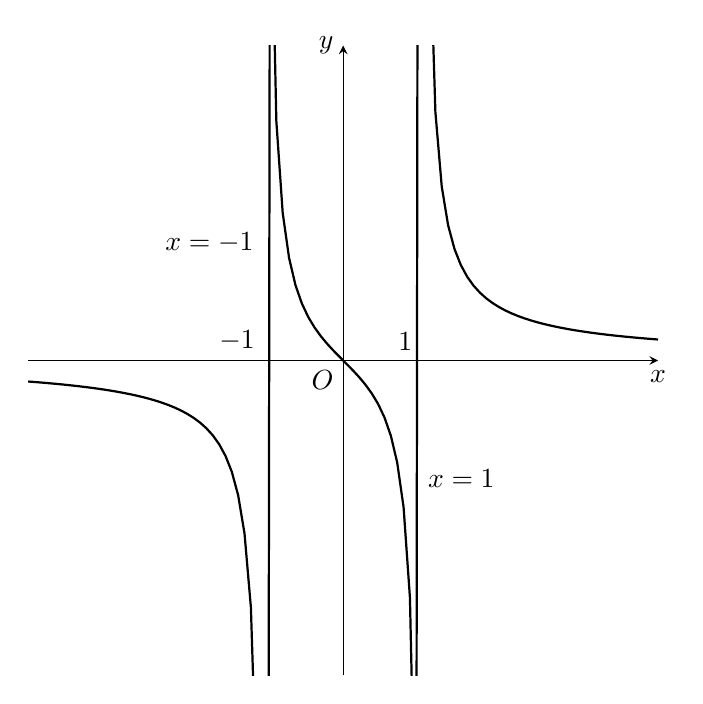
\begin{tikzpicture}[>=stealth]
\draw[->] (-4,0) --(4,0);
\draw[->](0,-4)--(0,4);
\draw (0,0) node[below left]{$O$};
\draw (4,0) node[below]{$x$};
\draw (0,4) node[left]{$y$};
\draw (1,0) node[above left]{$1$};
\draw (-1,0) node[above left]{$-1$};
\clip (-4,-4) rectangle(4,4);
\draw[thick,samples=100] plot[domain=-4:4]
(\x,{(\x)/((\x)^(2)-1)});
\draw (-1.7,1.5) node
{$x=-1$};
\draw (1.5,-1.5) node
{$x=1$};
\end{tikzpicture}
\end{center}
	\choice
	{Đồ thị hàm số chỉ có 2 đường tiệm cận đứng $x=-1$ và $x=1$}
	{\True Đồ thị hàm số có 3 đường tiệm cận}
	{Đồ thị hàm số có 4 đường tiệm cận}
	{Đồ thị hàm số có 2 đường tiệm cận đứng và 1 đường tiệm cận xiên}
	\loigiai{ Đồ thị hàm số có 2 đường tiệm cận đứng $x=-1$ và $x=1$ và một đường tiệm cận ngang $y=0$, hàm số không có đường tiệm cận xiên.}
\end{ex}
%-----------6-------------
\begin{ex}%[2D1N3-1]Câu 6
	Đồ thị hàm số $y=\dfrac{x-2}{x^{2}-4}$ có mấy đường tiệm cận?
	\choice
	{$3$}
	{$1$}
	{\True$2$}
	{$0$}
	\loigiai{ Hàm số $y=\dfrac{x-2}{x^{2}-4}=\dfrac{x-2}{(x-2)(x+2)}=\dfrac{1}{x+2}$.\\
	$\heva{&\displaystyle\lim_{x\to +\infty }\dfrac{1}{x+2}=0\\&
	\displaystyle\lim_{x\to -\infty }\dfrac{1}{x+2}=0.}$\\
	Nên $y=0$ là đường tiệm cận ngang của hàm số, hàm số có tiệm cận ngang thì không có tiệm cận xiên.\\
	$\heva{&\displaystyle\lim_{x\to -2^- }\dfrac{1}{x+2}= - \infty \\&
	\displaystyle\lim_{x\to -2^+ }\dfrac{1}{x+2}= + \infty.}$\\
	Nên $x=-2$ là đường tiệm cận đứng của hàm số.\\
	Vậy hàm số có hai đường tiệm cận.
	}
\end{ex}
%-----------7-------------
\begin{ex}%[2D1H3-1]Câu 7
	Tiệm cận xiên của hàm số $f(x)=\dfrac{x^2+x-1}{x}$ là 
	\choice
	{$y=x-1$}
	{$y=x-2$}
	{$y=x-3$}
	{\True$y=x+1$}
	\loigiai{ Gọi đường thẳng $y=ax+b, a\neq 0$  là đường tiệm cận xiên của hàm số\\
  Ta có $a=\displaystyle\lim_{x\to +\infty }\dfrac{\dfrac{x^2+x-1}{x}}{x}=1$.; 
	$b=\displaystyle\lim_{x\to +\infty }\left [  \dfrac{x^2+x-1}{x}-x \right ]=1$.\\
	Vậy đường tiệm cận xiên cần tìm của hàm số $f(x)$  có phương trình $y=x+1$.}
\end{ex}
%-----------8-------------
\begin{ex}%[2D1H3-1]Câu 8
	Đồ thị sau là của hàm số nào sau đây
	\begin{center}
		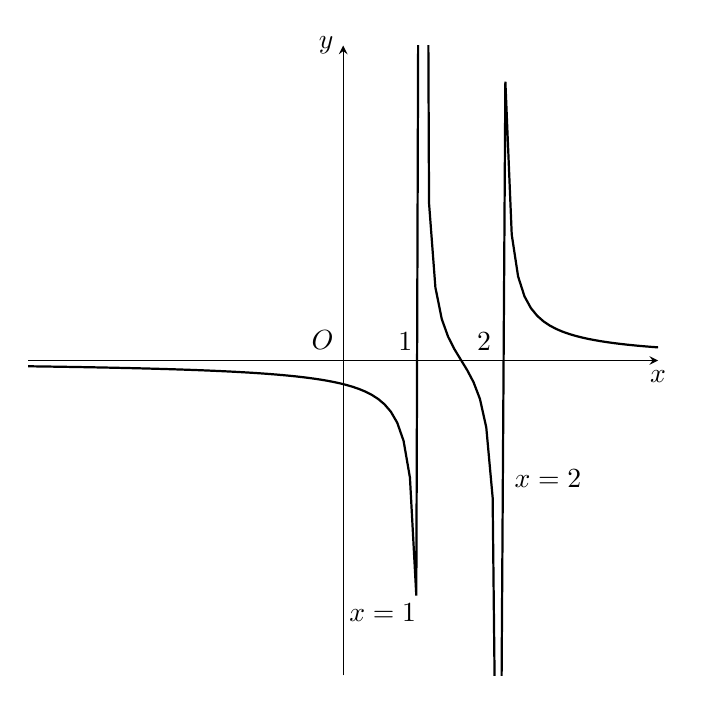
\begin{tikzpicture}[>=stealth]
			\draw[->] (-4,0) --(4,0);
			\draw[->](0,-4)--(0,4);
			\draw (0,0.5) node[below left]{$O$};
			\draw (4,0) node[below]{$x$};
			\draw (0,4) node[left]{$y$};
			\draw (1,0) node[above left]{$1$};
			\draw (2,0) node[above left]{$2$};
			\clip (-4,-4) rectangle(4,4);
			\draw[thick,samples=100] plot[domain=-4:4]
			(\x,{(2*(\x)-3)/(5*(\x)^(2)-15*\x+10)});
			\draw (2.6,-1.5) node
			{$x=2$};
			\draw (0.5,-3.2) node
			{$x=1$};
		\end{tikzpicture}
	\end{center}
	\choice
	{$\dfrac{2x^2+3}{5x^2-15x+10}$}
	{$\dfrac{2x-3}{x^2-5x+6}$}
	{\True $\dfrac{2x-3}{5x^2-15x+10}$}
	{$\dfrac{2x-3}{x^2+x-6}$}
	\loigiai{ Dựa vào đồ thị hàm số ta thấy có hai tiệm cận đứng là $x=1$ và $x=2$ loại hai đáp án có hàm số $\dfrac{2x-3}{x^2-5x+6}$ và $\dfrac{2x-3}{x^2+x-6}$, hàm số có đường tiệm cận ngang là $y=0$ vậy loại đáp án có hàm số $\dfrac{2x^2+3}{5x^2-15x+10}$.
	}
\end{ex}
%-----------9-------------
\begin{ex}%[2D1H3-1]Câu 9
	Bảng biến thiên sau là của đồ thị hàm số nào sau đây
	\begin{center}
	\begin{center}
	
\begin{tikzpicture}
		\tkzTabInit[nocadre,lgt=1.5,espcl=4,deltacl=.5]
		{$x$/0.7, $f’(x)$/0.7, $f(x)$/2}
		{$-\infty$,$1$,$+\infty$}
		\tkzTabLine{,-,d,-,}
		\tkzTabVar{+/$+\infty$,-D+/ $-\infty$/$+\infty$,-/$-\infty$}
	\end{tikzpicture}
\end{center}
\end{center}
	\choice
	{$y=\dfrac{x+1}{x-1}$}
	{\True$y=\dfrac{-x^2+2x}{x-1}$}
	{$y=\dfrac{-x^2+x}{x-1}$}
	{$y=\dfrac{x+2}{2x-2}$}
	\loigiai{ Dựa vào bảng biến thiên ta có tiệm cận đứng là $x=1$, ta lại có $\displaystyle\lim_{x\to +\infty }f(x)=-\infty$ và  $\displaystyle\lim_{x\to -\infty }f(x)=+\infty$ nên hàm số không có tiệm cận ngang loại đáp án $y=\dfrac{x+1}{x-1}$ và $y=\dfrac{x+2}{2x-2}$,\\
	loại đáp án $y=\dfrac{-x^2+x}{x-1}$ vì $y=\dfrac{-x^2+x}{x-1}=\dfrac{-1}{x-1}$ nên $\displaystyle\lim_{x\to +\infty }\dfrac{-1}{x-1}=0$ không phù hợp với bảng biến thiên.}
\end{ex}
%-----------10-------------
\begin{ex}%[2D1V3-1]Câu 10
Đồ thị hàm số $y=\dfrac{2x}{\sqrt{x^2-1}}$ có số đường tiệm cận là
	\choice
	{$2$}
	{$1$}
	{$3$}
	{\True$4$}
	\loigiai{Ta có\\ $\displaystyle\lim_{x\to +\infty }\dfrac{2x}{\sqrt{x^2-1}}=\displaystyle\lim_{x\to +\infty }\dfrac{2x}{|x|\sqrt{1-\dfrac{1}{x^2}}}=\displaystyle\lim_{x\to +\infty }\dfrac{2x}{x\sqrt{1-\dfrac{1}{x^2}}}=\displaystyle\lim_{x\to +\infty }\dfrac{2}{\sqrt{1-\dfrac{1}{x^2}}}=2$.\\
	$\displaystyle\lim_{x\to -\infty }\dfrac{2x}{\sqrt{x^2-1}}=\displaystyle\lim_{x\to -\infty }\dfrac{2x}{|x|\sqrt{1-\dfrac{1}{x^2}}}=\displaystyle\lim_{x\to -\infty }\dfrac{2x}{-x\sqrt{1-\dfrac{1}{x^2}}}=\displaystyle\lim_{x\to -\infty }\dfrac{-2}{\sqrt{1-\dfrac{1}{x^2}}}=-2$.\\
	Nên $y=-2$ và $y=2$ là hai đường tiệm cận ngang.\\
	Có $\displaystyle\lim_{x\to 1^-}y=\displaystyle\lim_{x\to (-1)^-}\dfrac{2x}{\sqrt{x^2-1}}=-\infty$; $ \displaystyle\lim_{x\to 1^+}y=\displaystyle\lim_{x\to 1^+}\dfrac{2x}{\sqrt{x^2-1}}=+\infty$.\\
	 Nên đồ thị hàm số có hai tiệm cận đứng $x=-1$ và $x=1$.\\
	 Vậy đồ thị hàm số có 4 tiệm cận.}
\end{ex}
%----------11------
\begin{ex}%[2D1V3-1]Câu 7
	Biết rằng đồ thị hàm só $y=\dfrac{(a-3)x+a+2025}{x-(b+3)}$ nhận trục hoành làm tiệm cận ngang và trục tung làm tiệm cận đứng. khi đó giá của $a+b$ là
	\choice
	{$3$}
	{$-3$}
	{\True $0$}
	{$6$}
	\loigiai{$\heva{&\displaystyle\lim_{x\to +\infty}\dfrac{(a-3)x+a+2025}{x-(b+3)}=a-3&\\&\displaystyle\lim_{x\to -\infty}\dfrac{(a-3)x+a+2025}{x-(b+3)}=a-3.}$\\
	$\heva{&\displaystyle\lim_{x\to (b+3)^-}\dfrac{(a-3)x+a+2025}{x-(b+3)}=+\infty\\&\displaystyle\lim_{x\to (b+3)^+}\dfrac{(a-3)x+a+2025}{x-(b+3)}=-\infty.}$\\
	$\to $ Đồ thị hàm số có tiệm cận ngang là $y=a-3$, tiệm cận đứng là $x=b+3$.\\
	theo bài ra, ta có $a-3=b+3=0\to a=3,b=-3 \to a+b=0$.}
\end{ex}
%----------12--------
\begin{ex}%[2D1V3-1]Câu 12
	Giao điểm của hai đường tiệm cận của đồ thị hàm số nào dưới đây nằm trên đường thẳng $d:y=x$
	\choice
	{$y=\dfrac{2x-1}{x+3}$}
	{\True$y=\dfrac{x+4}{x-1}$}
	{$y=\dfrac{2x+1}{x+2}$}
	{$\dfrac{1}{x+3}$}
	\loigiai{
		Đáp án $y=\dfrac{2x-1}{x+3}$ có giao hai đường tiệm tiệm cận là $(-3;2)\notin d$\\
		Đáp án $y=\dfrac{x+4}{x-1}$ có giao hai đường tiệm cận là $(1;1)\in d$\\
		Đáp án $y=\dfrac{2x+1}{x+2}$ có giao hai đường tiệm cận là $(-2;2)\notin d$\\
		Đáp án $\dfrac{1}{x+3}$ có giao hai đường tiệm cận là $(-3;0)\notin d$\\
	}
\end{ex}
\Closesolutionfile{ans}
\indapan{6}{ans/ans-0-B15}

\cauds%Câu đúng sai
\Opensolutionfile{ans}[ans/ans-0-B15-DS]
\begin{ex}%%[2D1N3-1]Câu 1
Cho các phát biểu sau
	\choiceTF
	{Nếu chỉ có điều kiện $\displaystyle\lim_{x\to a^+}f(x)=+\infty$ thì  đường thẳng $x=a$ không được gọi là đường tiệm cận đứng của đồ thị hàm số $f(x)$}
	{\True Đường thẳng $y=m$ được gọi là một đường tiệm cận ngang (hay tiệm cận ngang) của đồ thị hàm số $f(x)$ nếu  $\displaystyle\lim_{x\to -\infty}f(x)=m$ hoặc   $\displaystyle\lim_{x\to +\infty}f(x)=m$}
	{\True Đường thẳng $y=ax+b, a\neq0$, được gọi là tiệm cận xiên (hay tiệm cận xiên) của đồ thị hàm số $f(x)$ nếu $\displaystyle\lim_{x\to +\infty}[f(x)-(ax+b)]=0$}
	{\True Tiệm cận xiên $y=ax+b, a\neq0$ của $f(x)$ với hệ số $a=\displaystyle\lim_{x\to +\infty}\dfrac{f(x)}{x}$}
	\loigiai{
		\begin{itemchoice}
			\itemch Sai. Đường thẳng $x=a$ được gọi là một đường tiệm cận đứng của đồ thị hàm số $f(x)$ nếu ít nhất một trong các điều kiện sau thỏa mãn:\\ $\displaystyle\lim_{x\to a^-}f(x)=+\infty$; $\displaystyle\lim_{x\to a^+}f(x)=+\infty$; $\displaystyle\lim_{x\to a^-}f(x)=-\infty$; $\displaystyle\lim_{x\to a^+}f(x)=-\infty$.
			\itemch Đúng. Đường thẳng $y=m$ được gọi là một đường tiệm cận ngang (hay tiệm cận ngang) của đồ thị hàm số $f(x)$ nếu  $\displaystyle\lim_{x\to -\infty}f(x)=m$ hoặc   $\displaystyle\lim_{x\to +\infty}f(x)=m$.
			\itemch Đúng. Đường thẳng $y=ax+b, a\neq0$, được gọi là tiệm cận xiên (hay tiệm cận xiên) của đồ thị hàm số $f(x)$ nếu $\displaystyle\lim_{x\to +\infty}[f(x)-(ax+b)]=0$ hoặc $\displaystyle\lim_{x\to -\infty}[f(x)-(ax+b)]=0$.
			\itemch Đúng. Tiệm cận xiên $y=ax+b, a\neq0$ của $f(x)$\\ với hệ số $a=\displaystyle\lim_{x\to +\infty}\dfrac{f(x)}{x}$, $b=\displaystyle\lim_{x\to +\infty}[f(x)-ax]$.
		\end{itemchoice}
	}
\end{ex}

\begin{ex}%%[2D1H3-1]Câu 2
Cho hàm số $y=\dfrac{3(x^2+1)(x-3)}{(x+1)^3}$
	\choiceTF
	{ Hàm số không có tiệm cận ngang}
	{\True Hàm số có đúng một tiệm cận ngang}
	{ Hàm số có một tiệm cận xiên}
	{Hàm số không có tiệm cận đứng}
	\loigiai{
		\begin{itemchoice}
			\itemch Sai. $\displaystyle\lim_{x\to \pm \infty}\dfrac{3(x^2+1)(x-3)}{(x+1)^3}=\displaystyle\lim_{x\to \pm \infty}\dfrac{3\left (1+\dfrac{1}{x^2} \right )\left ( 1-\dfrac{3}{x} \right )}{1+\dfrac{3}{x}+\dfrac{3}{x^2}+\dfrac{1}{x^3}} =3$.\\
			Hàm số có đúng một tiệm cận ngang $y=3$.
			\itemch Đúng. Dựa vào đáp án của ý a.
			\itemch Sai. Hàm số có tiệm cận ngang thì không có tiệm cận xiên.
			\itemch Sai.$\heva{&\displaystyle\lim_{x\to -1^-}\dfrac{3(x^2+1)(x-3)}{(x+1)^3}=+\infty.\\&
			\displaystyle\lim_{x\to -1^+}\dfrac{3(x^2+1)(x-3)}{(x+1)^3}=+\infty.} $\\
		     Vậy hàm số có một tiệm cận đứng $x=-1$.
		\end{itemchoice}
	}
\end{ex}

\begin{ex}%%[2D1H3-1]Câu 3
	Cho đồ thị của hàm số $f(x)$ như hình sau
\begin{center}
	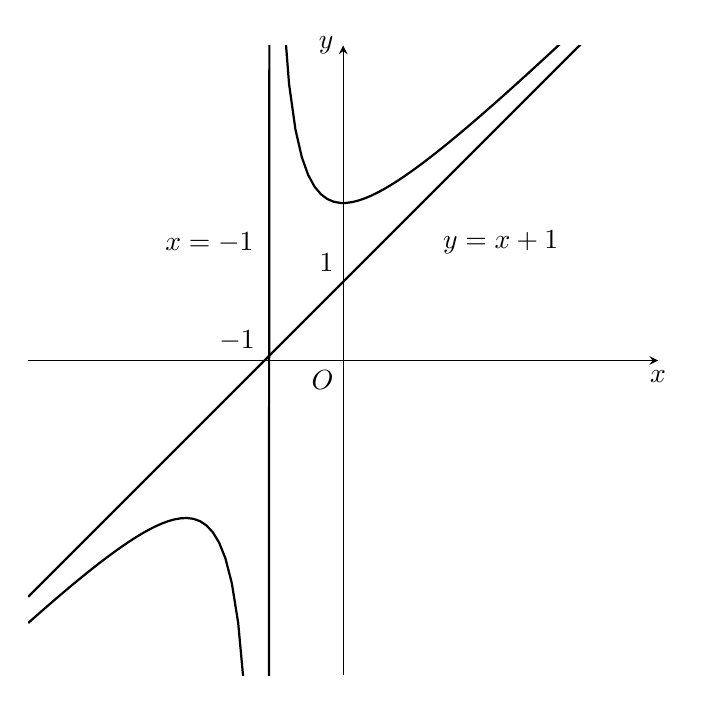
\begin{tikzpicture}[>=stealth]
		\draw[->] (-4,0) --(4,0);
		\draw[->](0,-4)--(0,4);
		\draw (0,0) node[below left]{$O$};
		\draw (4,0) node[below]{$x$};
		\draw (0,4) node[left]{$y$};
		\draw (-1,0) node[above left]{$-1$};
		\draw (0,1) node[above left]{$1$};
		\clip (-4,-4) rectangle(4,4);
		\draw[thick,samples=100] plot[domain=-4:4]
		(\x,{((\x)^2+2*\x+2)/((\x)+1)});
		\draw[thick,samples=100] plot[domain=-4:4]
		(\x,{\x+1});
		\draw (-1.7,1.5) node
		{$x=-1$};
		\draw (2,1.5) node
		{$y=x+1$};
	\end{tikzpicture}
\end{center}
	\choiceTF
	{ $y=x+1$ là đường tiệm cận ngang của hàm số $f(x)$}
	{\True hàm số $f(x)$ có một đường tiệm cận đứng và một đường tiệm cận xiên }
	{\True đồ thị hàm số có phương trình là $f(x)=\dfrac{x^2+2x+2}{x+1}$}
	{\True hàm số $f(x)$ có đường tiệm cận xiên là $y=x+1$}
	
	\loigiai{
		\begin{itemchoice}
			\itemch Sai. Dựa đồ thị hàm số của $f(x)$ hàm số không có tiệm cận ngang.
			\itemch Đúng. Dựa đồ thị hàm số của $f(x)$ hàm số có đường tiệm cận đứng $x=-1$.
			\itemch Đúng. Gọi $y=ax+b,a\neq0$ là đường tiệm cận xiên của $f(x)$\\
			$a=\displaystyle\lim_{x\to +\infty}\dfrac{f(x)}{x}=\displaystyle\lim_{x\to +\infty}\dfrac{\dfrac{x^2+2x+2}{x+1}}{x}=\displaystyle\lim_{x\to +\infty}\dfrac{x^2+2x+2}{x(x+1)}=1$.\\
			$b=\displaystyle\lim_{x\to +\infty}[f(x)-ax]=\displaystyle\lim_{x\to +\infty}\left [ f(x)\dfrac{x^2+2x+2}{x+1}-x\right ]=1$.\\
			Vậy $y=x+1$ là đường tiệm cận xiên của hàm số $f(x)$.\\
			$\heva{&\displaystyle\lim_{x\to -1^+}\dfrac{x^2+2x+2}{x+1}= +\infty\\&
			\displaystyle\lim_{x\to -1^-}\dfrac{x^2+2x+2}{x+1}= -\infty.}$\\
		vậy $x=-1$ là đường tiệm cận đứng.
			\itemch Đúng. Dựa vào đồ thị, đường thẳng $y=x+1$ là đường tiệm cận xiên của $f(x)$.
		\end{itemchoice}
	}
\end{ex}
\begin{ex}%%[2D1V3-1]Câu 4
Đồ thị trong hình là của hàm số $y=\dfrac{ax+b}{x+c}.(a,b,c\in\mathbb{R})$. Khi đó tổng $a+b+c$ bằng 
\begin{center}
	\begin{tikzpicture}[>=stealth]
		\draw[->] (-4,0) --(4,0);
		\draw[->](0,-4)--(0,4);
		\draw (0,0) node[below left]{$O$};
		\draw (4,0) node[below]{$x$};
		\draw (0,4) node[left]{$y$};
		\draw (1,0) node[above left]{$1$};
		\draw (0,-1) node[above left]{$-1$};
		\clip (-4,-4) rectangle(4,4);
		\draw[thick,samples=100] plot[domain=-4:4]
		(\x,{(-(\x)+2)/((\x)-1)});
		\draw[thick,samples=100] plot[domain=-4:4]
		(\x,-1);
		\draw (2,-2) node
		{$x=1$};
	\end{tikzpicture}
\end{center}
	\choiceTF
	{ \True Hàm số có tiệm cận ngang là $y=-1$}
	{\True Hàm số có tiệm cận đứng là $x=1$}
	{\True  $a+b+c=0$}
	{Hàm số đồng biến trên các khoảng xác định}
	\loigiai{
		\begin{itemchoice}
			\itemch Đúng. Dựa vào đồ thị ta thấy đường thẳng $y=-1$ là tiệm cận ngang.
			\itemch Đúng. Dựa vào đồ thị ta thấy đường thẳng $x=1$ là tiệm cận đứng.
			\itemch Đúng. Dựa vào đồ thị hàm số có tiệm cận ngang $y=-1\to  a=-1$, tiệm cận đứng $x=1\to  c=-1$ và hàm số đi qua điểm $(2;0)$ nên $0=\dfrac{-2+b}{2-1} \to  b=2$.\\ vậy $a+b+c=-1+2-1=0$.
			\itemch Sai. Ta có $y=\dfrac{-x+2}{x-1} \to  y'=\dfrac{-1}{(x-1)^2}\leq0$, vậy hàm số nghịch biến trên các khoảng xác định.
		\end{itemchoice}
	}
\end{ex}



\Closesolutionfile{ans}
\indapan{3}{ans/ans-0-B15-DS}

\Opensolutionfile{ans}[ans/ans-0-B15-KQ]

\caukq
\begin{ex}%%[2D1H3-1]Câu 1
Đồ thị hàm số $y=\dfrac{x-3}{x^2+x-2}$ có bao nhiêu đường tiệm cận đứng?
	\shortans{$2$}
	\loigiai{ $\heva{&\displaystyle\lim_{x\to 1^+}y=\dfrac{x-3}{x^2+x-2}= -\infty\\&
		\displaystyle\lim_{x\to 1^-}y=\dfrac{x-3}{x^2+x-2}= +\infty.}$\\
		Nên $x=1$ là đường tiệm cận đứng của hàm số.\\
		$\heva{\displaystyle\lim_{x\to 2^+}y=\dfrac{x-3}{x^2+x-2}= +\infty\\
		\displaystyle\lim_{x\to 2^-}y=\dfrac{x-3}{x^2+x-2}= -\infty.}$\\
		Nên $x=-2$ là đường tiệm cận đứng của hàm số.\\
		Vậy hàm số có hai đường tiệm cận đứng.
	}
\end{ex}

\begin{ex}%[2D1H3-1]Câu 2
	Cho hàm số $y=f(x)$ xác định trên $\mathbb{R}\setminus\{-1\}$ có bảng biến thiên như hình dưới đây, hàm số có bao nhiêu tiệm cận ngang
	\begin{center}
	
\begin{tikzpicture}
		\tkzTabInit[nocadre,lgt=1.5,espcl=2,deltacl=.5]
		{$x$/0.7, $f’(x)$/0.7, $f(x)$/2}
		{$-\infty$,$-1$,$2$,$+\infty$}
		\tkzTabLine{,+,d,-,0,+,}
		\tkzTabVar{-/$-1$,+D+/$+\infty$/$+\infty$, -/$0$,+/$+\infty$} 
	\end{tikzpicture}
	\end{center}
	\shortans{$1$}
	\loigiai{ Dựa vào bảng biến thiên ta thấy $\displaystyle\lim_{x\to -\infty}f(x)=-1$ nên hàm số có đường tiệm cận ngang $y=-1$. Nên hàm số có 1 tiệm cận ngang.}
\end{ex}

\begin{ex}%[2D1V3-1]Câu 3
Cho hàm số $f(x)$ xác định và liên tục trên $\mathbb{R}\setminus\{-1\}$, có bảng biến thiên như sau:

	\begin{center}
	
\begin{tikzpicture}
		\tkzTabInit[nocadre,lgt=1.5,espcl=3,deltacl=.5]
		{$x$/0.7, $f’(x)$/0.7, $f(x)$/2}
		{$-\infty$,$-1$,$+\infty$}
		\tkzTabLine{,-,d,-,}
		\tkzTabVar{+/$2$,-D+/$-\infty$/$+\infty$,-/$-2$} 
	\end{tikzpicture}
	\end{center}
	Hỏi đồ thị hàm số $y=\dfrac{1}{f(x)}$ có tất cả bao nhiêu đường tiệm cận đứng và tiệm cận ngang?
	\shortans{$4$}
	\loigiai{ Dựa vào BBT ta có $\displaystyle\lim_{x\to -\infty}f(x)=2$, $\displaystyle\lim_{x\to +\infty}f(x)=-2$, $\displaystyle\lim_{x\to -1^-}f(x)=-\infty$, $\displaystyle\lim_{x\to -1^+}f(x)=+\infty$.\\
		Đặt $y=g(x)=\dfrac{1}{f(x)}$ ta có\\
		$\displaystyle\lim_{x\to +\infty}g(x)=\displaystyle\lim_{x\to +\infty}\dfrac{1}{f(x)}=\dfrac{-1}{2}\to y=\dfrac{-1}{2}$ là TCN của đồ thị hàm số $y=g(x)=\dfrac{1}{f(x)}$.\\
		$\displaystyle\lim_{x\to -\infty}g(x)=\displaystyle\lim_{x\to -\infty}\dfrac{1}{f(x)}=\dfrac{1}{2}\to y=\dfrac{1}{2}$ là TCN của đồ thị hàm số $y=g(x)=\dfrac{1}{f(x)}$.\\
		$\displaystyle\lim_{x\to -1}g(x)=\displaystyle\lim_{x\to -1}\dfrac{1}{f(x)}=0\to x=-1$ không là TCĐ của đồ thị hàm số $y=g(x)=\dfrac{1}{f(x)}$.\\
		Xét phương trình $f(x)=0$\\
		
		\begin{center}
			\begin{tikzpicture}
				\tkzTabInit[nocadre,lgt=1.5,espcl=3,deltacl=.5]
				{$x$/0.7, $f’(x)$/0.7, $f(x)$/2}
				{$-\infty$,$-1$,$+\infty$}
				\tkzTabLine{,+,d,-,}
				\tkzTabVar{+/$2$,-D+/$-\infty$/$+\infty$,-/$-2$} 
				\draw[red] (2,-2.3)--(9,-2.3) node[above]{$y=0$};
			\end{tikzpicture}
		\end{center}
		
		 dựa vào BBT ta thấy phương trình có hai nghiệm phân biệt thỏa mãn khác $-1$.
		Do đó đồ thị hàm số $y=g(x)=\dfrac{1}{f(x)}$ có 2 TCĐ.\\
		Vậy đồ thị hàm số $y=g(x)=\dfrac{1}{f(x)}$ có tất cả 4 đường tiệm cận.
	
	}
\end{ex}

\begin{ex}%%[2D1V3-1]Câu 4
	Có bao nhiêu giá trị nguyên của tham số $m$ thuộc đoạn $[-2025;2025]$ để hàm số $y=\dfrac{x+2}{\sqrt{x^2-4x+m}}$ có hai tiệm cận đứng?
	\shortans{$2028$}
	\loigiai{
	Hàm số có hai tiệm cận đứng khi $x^2-4x+m=0$ có hai nghiệm phân biệt khác $-2$ $\Leftrightarrow \heva{& m\neq-2\\&m<4}\to m\in [-2025;4)\setminus\{-2\}.$}
\end{ex}


\begin{ex}%[2D1C3-1]Câu 5
 Số giá trị nguyên của tham số $m$ để hàm số $y=\dfrac{1+\sqrt{x+1}}{x^2-(1-m)x+2m}$ có 3 đường tiệm cận (bao gồm tiệm cận đứng và tiệm cận ngang) là
	\shortans{$2$}
	\loigiai{
	 Điều kiện xác định $\heva{&x\geq-1\\&x^2-(1-m)x+2m\neq0}.$\\ 
	 Ta có $y=\dfrac{1+\sqrt{x+1}}{x^2-(1-m)x+2m}$.\\
	  Đồ thị hàm số $y=\dfrac{1+\sqrt{x+1}}{x^2-(1-m)x+2m}.(x\geq-1)$ có tiệm cận ngang là đường thẳng $y=0$.\\
	  Do đó để hàm số có 3 đường tiệm cận thì hàm số phải có 2 tiệm cận đứng\\
	  $\to x^2-(1-m)x+2m=0$ có 2 nghiệm phân biệt lớn hơn $-1$\\
	  $\Leftrightarrow \heva{&\Delta>0\\&(x_1+1)(x_2+1)>0\\&x_1+1+x_2+1>0}\Leftrightarrow \heva{&(1-m)^2-8m>0\\&x_1x_2+(x_1+x_2)+1>0\\&x_1+x_2+x_2+2>0}\Leftrightarrow \heva{&(1-m)^2-8m>0\\&2m+1-m+1>0\\&1-m+2>0}$\\
	  $\Leftrightarrow \heva{&1-2m+m^2-8m>0\\&m+2>0\\&m<3}\Leftrightarrow \heva{&m^2-10m+1>0\\&m>-2\\&m<3}\Leftrightarrow \heva{&\hoac{&m>5+2\sqrt{6}\\&m<5-2\sqrt{6}}\\&-2<m<3}$ \\$ \Leftrightarrow -2<m<5-2\sqrt{6}$.\\
	  Vậy $m\in\{-1;0\}$ suy ra có 2 giá trị $m$ thảo mãn.
	}
\end{ex}

\begin{ex}%[2D1C3-1]Câu 6
Cho hàm đa thức bậc ba $y=f(x)$ có đồ thị như hình vẽ
\begin{center}
	\begin{tikzpicture}[>=stealth]
		\draw[->] (-4,0) --(4,0);
		\draw[->](0,-4)--(0,4);
		\draw (0,0.5) node[below left]{$O$};
		\draw (4,0) node[below]{$x$};
		\draw (0,4) node[left]{$y$};
		\draw (2,0) node[above left]{$2$};
		\draw (-1,0) node[above left]{$-1$};
		\draw[dashed] (0,-2)
		node[left]{$-2$} -- (1,-2) --
		(1,0) node[above]{$1$};
		\clip (-4,-4) rectangle(4,4);
		\draw[thick,samples=100] plot[domain=-4:4]
		(\x,{(1/2)*(\x)^3-(3/2)*\x-1});
	\end{tikzpicture}
\end{center}
Tổng số đường tiệm cận ngang và tiệm cận đứng của đồ thị $y=\dfrac{(x+1)(x^2-1)}{f(x)}$ là
	\shortans{$3$}
	\loigiai{ Hàm số có dạng $f(x)=ax^3+bx^2+cx-1$ (vì là hàm bậc ba cắt trục tung tại điểm có tung độ $-1$)\\
    Đồ thị hàm số đã cho đi qua các điểm có tọa độ là $(-1;0)$, $(1;-2)$, $(2;0)$ \\
    $\to \heva{&8a+4b+2c=1\\& -a+b-c=1 \\&a+b+c=-1}\Leftrightarrow \heva{&a=\dfrac{1}{2}\\&b=0 \\&c=\dfrac{-3}{2}.}$\\
    $\to f(x)=\dfrac{1}{2}x^3-\dfrac{3}{2}x-1=\dfrac{1}{2}(x-1)^2(x-2)$.\\
    Khi đó $y=\dfrac{(x+1)(x^2-1)}{f(x)}=\dfrac{(x+1)(x^2-1)}{\dfrac{1}{2}(x-1)^2(x-2)}=\dfrac{2(x+1)^2}{(x-1)(x-2)}$.\\
    Đồ thị hàm số trên có tiệm cận ngang $y=2$ và tiệm cận đứng là $x=1,x=2$.\\
     Vậy đồ thị hàm số $y=\dfrac{(x+1)(x^2-1)}{f(x)}$ có 3 đường tiệm cận.
	}
\end{ex}
\Closesolutionfile{ans}
\indapan{6}{ans/ans-0-B15-KQ}